The details of the numerical setup are presented in Section \ref{sec_fspq1p0}.
The main difference resides in the Schur complement approach to solve the 
Stokes system, as presented in Section \ref{sec_solvers} (see {\bf solver\_cg}).
This iterative solver is very easy to implement once the blocks $\K$ and $\G$, 
as well as the rhs vectors $f$ and $h$ have been built. 



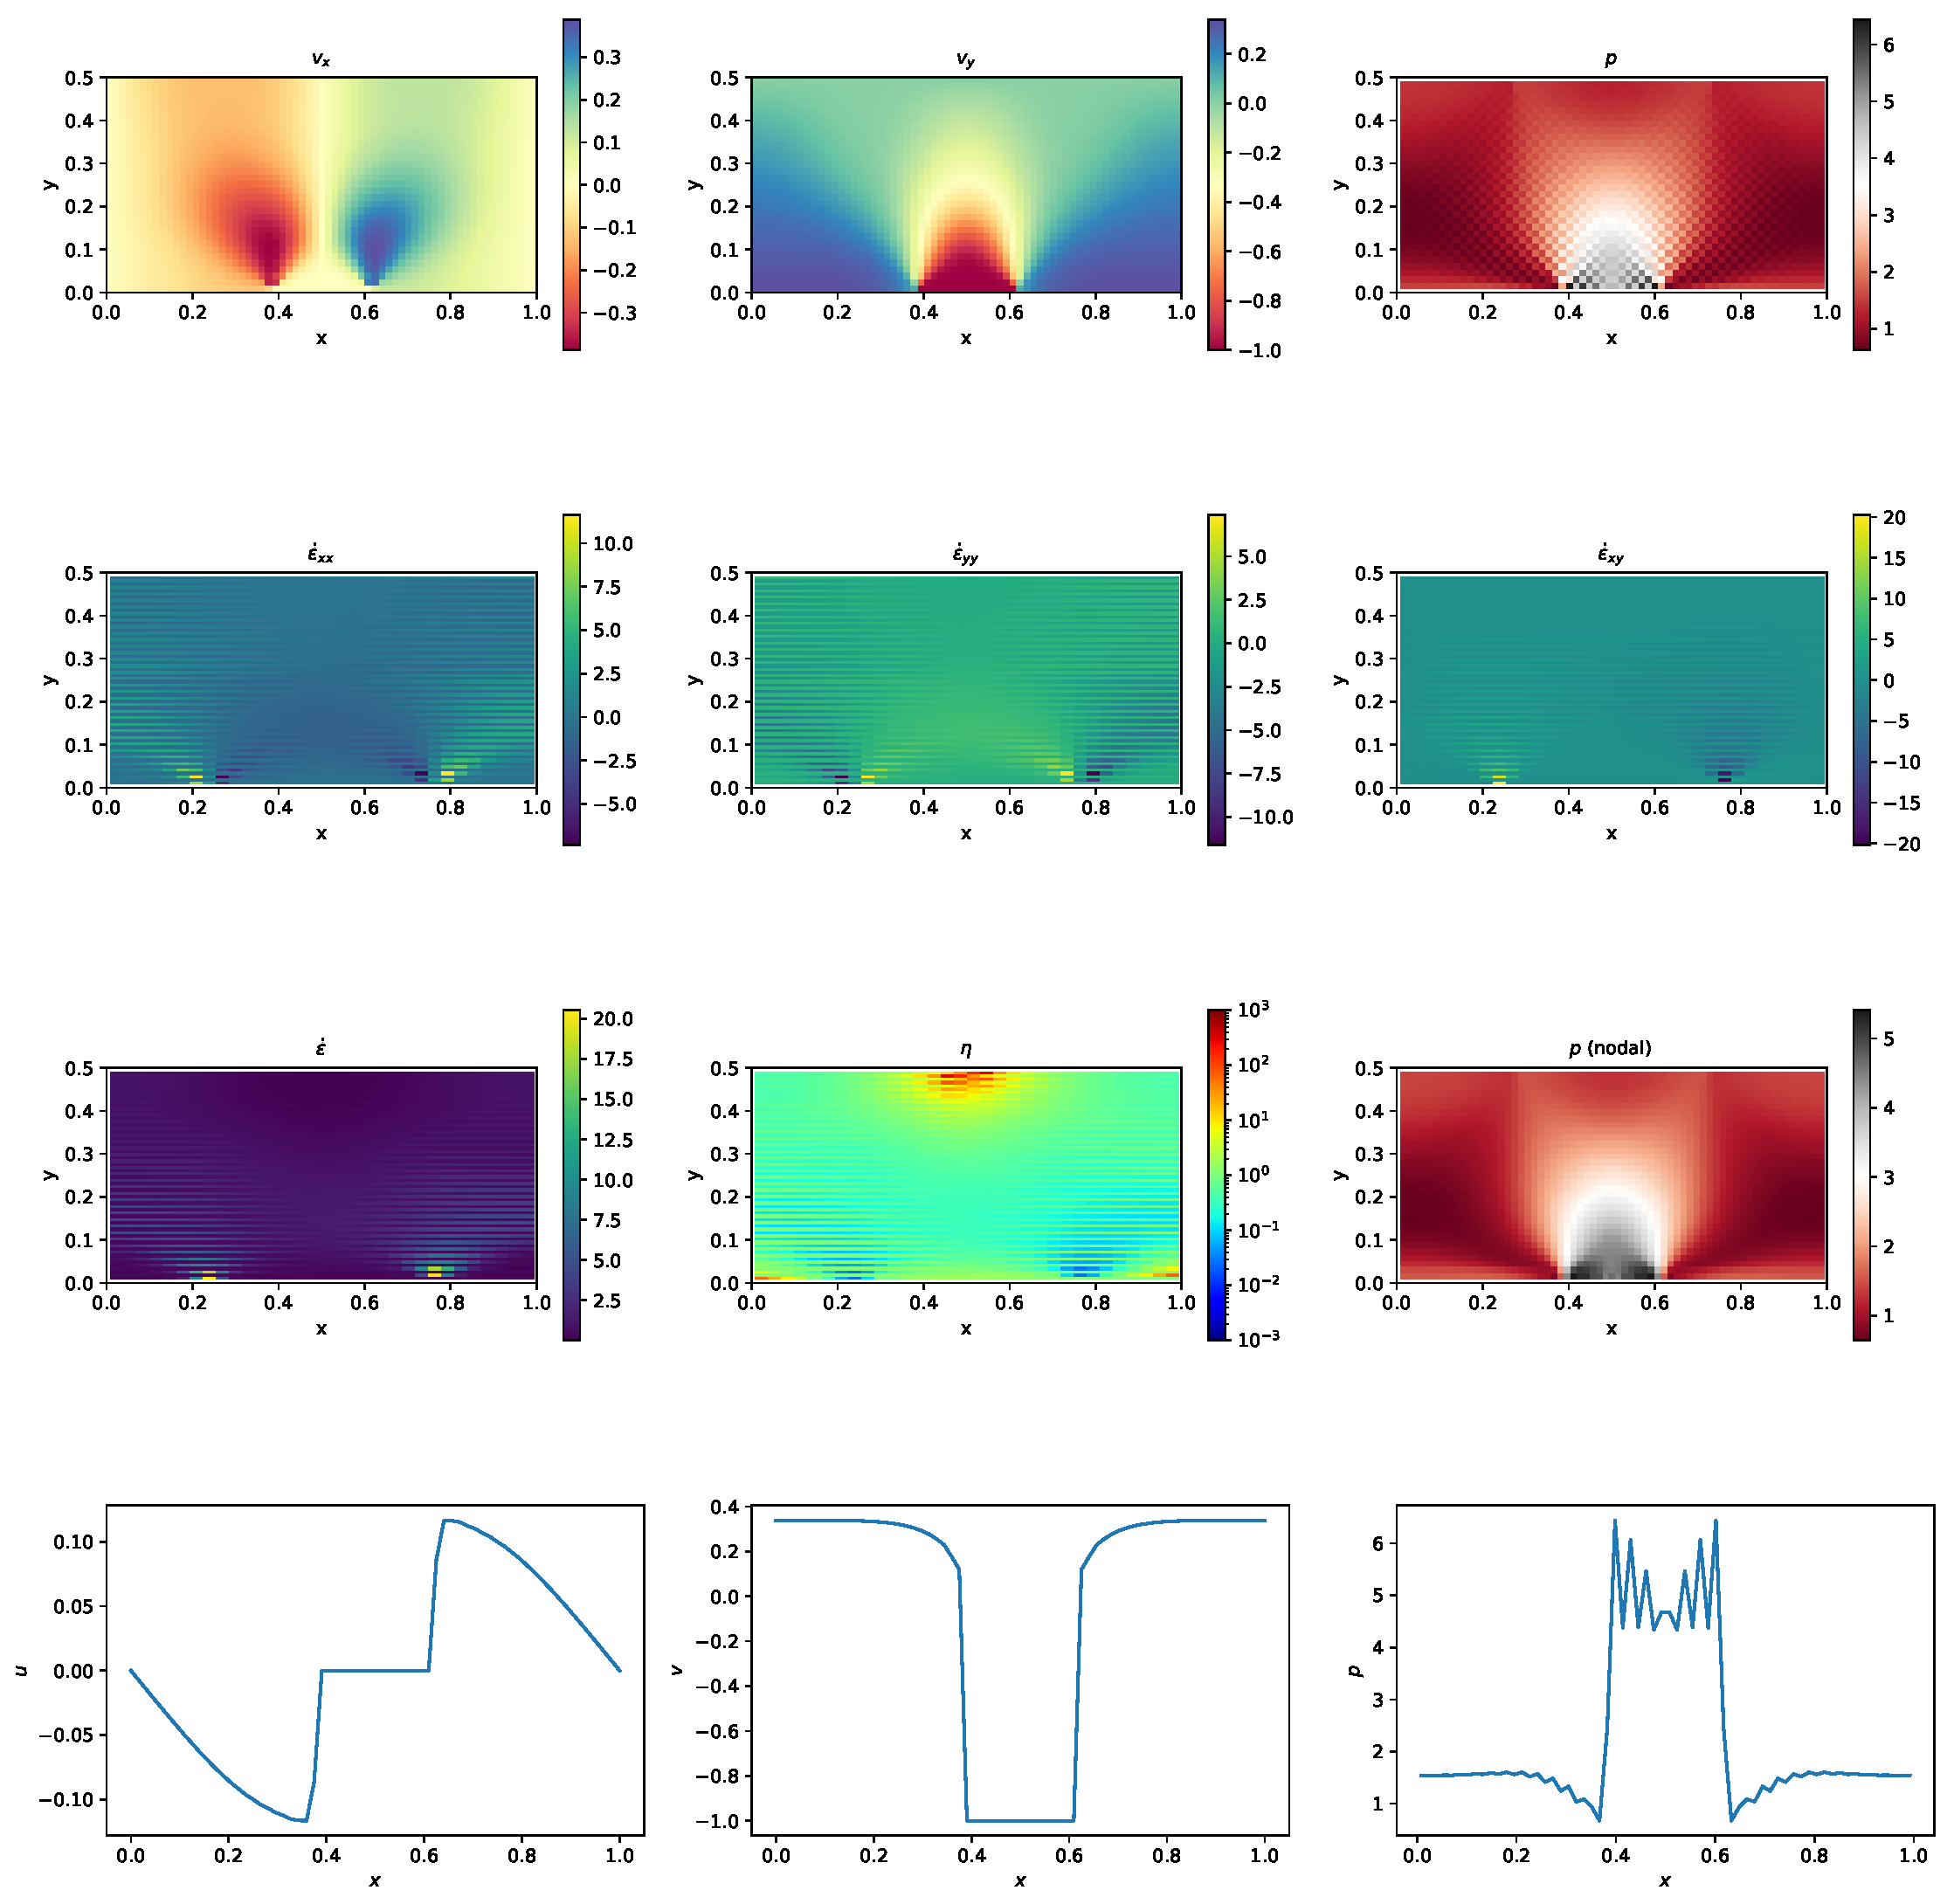
\includegraphics[width=16cm]{/home/cedrict/Desktop/FIELDSTONE/fieldstone/python_codes/fieldstone_saddlepoint_q1p0_schurcomplement/images/solution.pdf}

Rather interestingly the pressure checkerboard modes are not nearly as present as in Section \ref{sec_fspq1p0} which uses a full matrix approach. 

Looking at the discretisation errors for velocity and pressure, we of course recover the same rates and values as in the full matrix case.

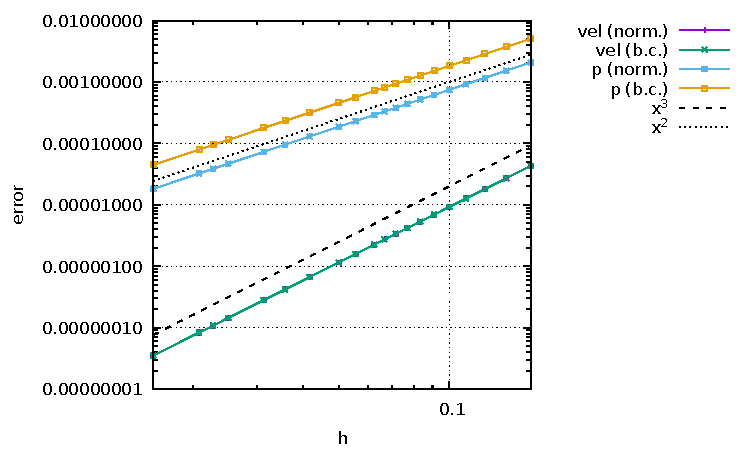
\includegraphics[width=16cm]{/home/cedrict/Desktop/FIELDSTONE/fieldstone/python_codes/fieldstone_saddlepoint_q1p0_schurcomplement/images/errors.pdf}

Finally, for each experiment the normalised residual (see {\bf solver\_cg}) was recorded. We see that 
all things equal the resolution has a strong influence on the number of iterations the solver must
perform to reach the required tolerance. This is one of the manifestations of the fact that the 
$Q_1 \times P_0$ element is not a stable element: the condition number of the matrix increases with 
resolution. We will see that this is not the case of stable elements such as $Q_2\times Q_1$.

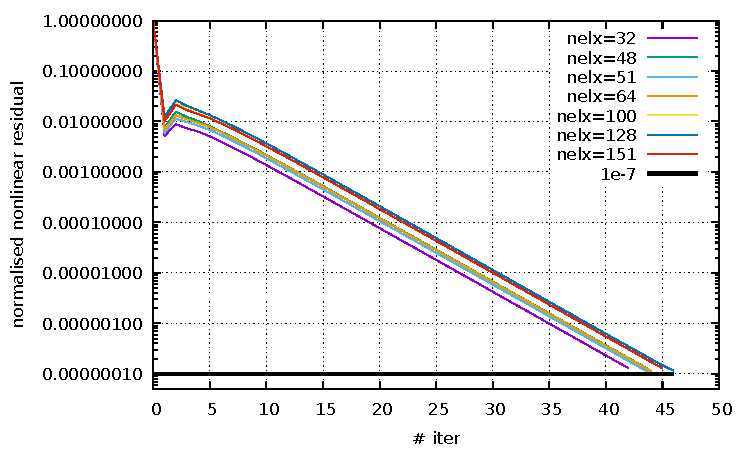
\includegraphics[width=16cm]{/home/cedrict/Desktop/FIELDSTONE/fieldstone/python_codes/fieldstone_saddlepoint_q1p0_schurcomplement/images/residual.pdf}
 
\fbox{
\parbox{10cm}{{\bf features}
\begin{itemize}
\item $Q_1\times P_0$ element \index{$Q_1 \times P_0$}
\item incompressible flow \index{incompressible flow}
\item mixed formulation \index{mixed formulation}
\item Schur complement approach \index{Schur complement approach}
\item isothermal \index{isothermal}
\item isoviscous \index{isoviscous}
\item analytical solution \index{analytical solution}
\end{itemize}
}}

\improvement{build S and have python compute its smallest and largest eigenvalues as a function of resolution?}
